\documentclass[9pt,shortpaper,twoside,web]{ieeecolor}
\usepackage{generic}
\usepackage{cite}
\usepackage{amsmath,amssymb,amsfonts}
\usepackage{algorithmic}
\usepackage{algorithm}
\usepackage{graphicx}
\usepackage{textcomp}
\usepackage{caption}
\usepackage{amssymb}
\def\BibTeX{{\rm B\kern-.05em{\sc i\kern-.025em b}\kern-.08em
    T\kern-.1667em\lower.7ex\hbox{E}\kern-.125emX}}
\markboth{\journalname, 2018}
{Author: Kemiao Huang, A Heuristic Approach to Capacitated Arc Routing Problem using Simulated Annealing (November 2018)}
\begin{document}
\title{\bigskip\bigskip A Heuristic Approach to Capacitated Arc Routing Problem using Simulated Annealing}
\author{Kemiao Huang, 11610728, \IEEEmembership{Undergraduate, CSE}}
\maketitle

\begin{abstract}
The capacitated arc routing problem (CARP) is a classical problem and it's popular for many years since its wide applications in society. The simulated annealing is a regular and well-known for heuristic in NP hard problem. In this paper, a simulated annealing based heuristic approach is proposed for CARP. The most difficult point for simulated annealing is to set the parameters to control the balance between time cost and mutation effectiveness. A novel time control is proposed for the simulated annealing to get the output before time out.
\end{abstract}

\begin{IEEEkeywords}
Capacitated arc routing problem (CARP), dynamic time control, local search, optimization, simulated annealing
\end{IEEEkeywords}

\section{Preliminaries}
\IEEEPARstart{T}{he} Objective of this project is to realize an effective algorithm to find a solution for CARP in certain time as good as possible.  

\subsection{Introduction}
\subsubsection{Problem Description}
Arc Routing is the process of selecting the best path in a network based on the route. There are many types of arc routing. Each one has different goal and heuristic. All of them are NP-hard problems. The capacipated arc routing problem is one of the branches of arc routing problem. It consists of an undirected graph with required edges and non-required edges. Each edge has its demand and cost. There are a number of vehicles with maximum   capacities. Each vehicle should starts from the depot node and tries to meet the demand of each edge and returns depot without exceeding the its capacity. The goal is to minimise the cost for the vehicles to meet all the demands on each edge.     

\subsubsection{Problem Application}
It is suitable to adopt the approach based on CARP in which demands are set on arcs. For example, urban waste collection[1], post delivery, mail delivery where demand is concentrated and road sweeping where road section itself is the target of service.

\section{Methodology}
To get the initial solution for simulated annealing heuristic, shortest path based path scanning is used. To realize the mutation for solutions, three classical moving operators are used, which are single insertion, swap and two-opt. To control the time cost of the whole procedure, rather than use sampling to set the parameter at the first time, a dynamic fixing approach is used during the simulated annealing process.
\subsection{Notations}
The input of CARP contains the vehicle capacity denoted by \textit{Q}, a mixed graph \textit{G} = (\textit{V, E, A}), with vertices denoted by \textit{V}, edges denoted by \textit{E} and required arcs denoted by \textit{A}. Moreover, the depot for the routing is denoted by \textit{D} and the shortest-distance matrix is denoted by \textit{S}.

\begin{figure}[!t]
\centering
\captionsetup{justification=centering}
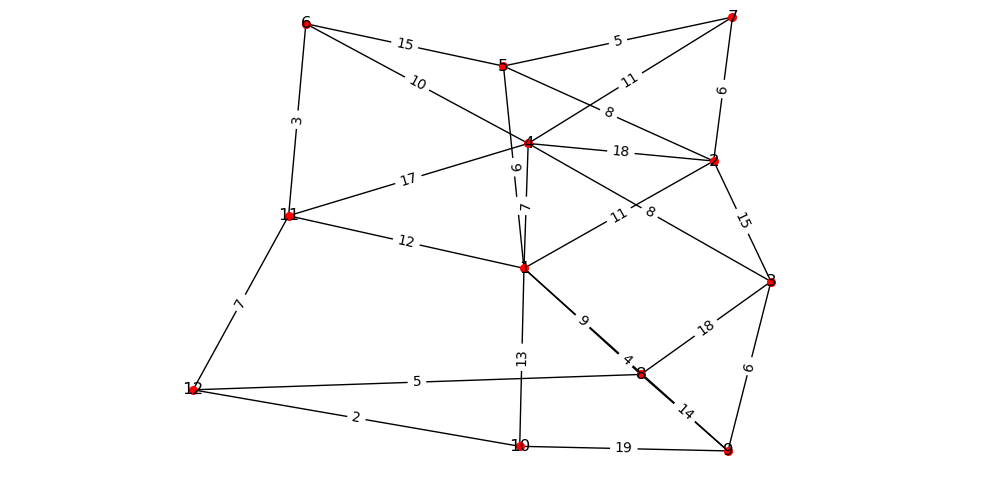
\includegraphics[width=\columnwidth]{gdb10.png}
\caption{The graph sample for CARP (gdb10)}
\label{fig1}
\end{figure}

\subsection{Data Structures}
\subsubsection{Shortest-Distance Matrix}
Since arc routing problem doesn't need the attribute for the vertices but the demand and cost of edges instead, the shortest-distance matrix is used without storing the graph information like connectivity, leaf and parent.
\subsubsection{List}
The python list is used for storing, inserting and popping the arcs, routes and solutions. 
\subsection{Model Design}
Basically, a CARP solution contains its route list and quality (i.e. total cost), a route contains a required arc list, load and cost, an arc contains its begin vertex, end vertex, demand and cost. For easier implementation, the arcs have fixed begin and end vertices with another boolean variable for declaring the direction of the arc. 

\begin{table}[ht]
\caption{Class Declaration}
\label{table}
\centering
\begin{tabular}{|l|l|}
\hline
Classes & Attributes \\ \hline
Arc & begin\_index, end\_index, load, cost, reverse \\ \hline
Route & required\_arc\_list, cost \\ \hline
Solution & route\_list, quality \\ \hline
\end{tabular}
\end{table}

Firstly, read the input file and build the corresponding arcs and set the basic parameters. Secondly, Floyd algorithm is used for constructing the n by n shortest-distance matrix. Next, the initial solution comes out from doing path scanning for all the required arcs. Then the iteration parameter for the simulated annealing is computed according to the remaining time and start annealing. The solution comes out by annealing is the best one. Finally, print the solution in the right format.

\subsection{Algorithms}

\subsubsection{Floyd Warshall Algorithm}
This algorithm is used to construct the shortest path between each vertex. By contrast, Dijkstra algorithm theoretically 
has smaller time complexity by using Fibonacci heap or pairing heap as its priority queue[3]. However, Floyd algorithm is more easily to implement and the difference of practical time cost is very small. Therefore, Floyd algorithm is chosen for this procedure.
\begin{algorithm}
 \caption{Floyd-Warshall}
 \begin{algorithmic}[h]
 \renewcommand{\algorithmicrequire}{\textbf{Input:}}
 \renewcommand{\algorithmicensure}{\textbf{Output:}}
 \REQUIRE $V$, $E$
 \ENSURE  shortest path matrix $S$\\ 
 \STATE $dist \gets n\times n$ array of minimum distances initialized to $\infty$ 
 \FOR{$v$ $\in$ $V$}
 \STATE $dist[u][v]\gets 0$
 \ENDFOR 
 \FOR{edge$(u,v)\in E$}
 \STATE $dist$[$u$][$v$] $\gets$ cost($u,v$)
 \ENDFOR
 \FOR {$k \gets 1$ to $n$}
 \FOR {$i \gets 1$ to $n$} 
 \FOR {$j \gets 1$ to $n$}
 \IF {$dist[u][v]>dist[i][k]+dist[k][j]$}
 \STATE $dist[u][v]\gets dist[i][k]+dist[k][j]$  
 \ENDIF
 \ENDFOR
 \ENDFOR
 \ENDFOR
 \RETURN $dist$
 \end{algorithmic} 
 \end{algorithm}

\subsubsection{Path Scanning}
In order to get the initial solution as good as possible in short time, the classical approach using path scanning is used. To increase the randomness and get better solution, the traditional five rules[2] for choosing the same distance arcs are not used. Instead, the arcs with the same distance from the current source are pure randomly chosen. The formal initial solution is come out by choosing the best of ten outputs of path scanning.

\begin{algorithm}
 \caption{Path Scanning}
 \begin{algorithmic}[h]
 \renewcommand{\algorithmicrequire}{\textbf{Input:}}
 \renewcommand{\algorithmicensure}{\textbf{Output:}}
 \REQUIRE required arc list $free$
 \ENSURE  route $R$\\ 
 \STATE $R \gets$ new empty route
 \STATE $i \gets D$
 \WHILE{\TRUE}
 \STATE $\overline{d}\gets\infty$ 
 \STATE $\overline{u}\gets\varnothing$
 \FOR{$u$ $\in$ $free$}
 \IF{$R.load+u.demand>Q$}
 \STATE \textbf{continue}
 \ENDIF
 \IF{$dist[i].begin<\overline{d}$}
 \STATE $\overline{d}\gets dist[i].begin$ 
 \STATE $\overline{u}\gets u$
 \STATE $reverse\gets\FALSE$
 \ELSIF {$dist[i].end<\overline{d}$}
 \STATE $\overline{d}\gets dist[i].end$ 
 \STATE $\overline{u}\gets u$
 \STATE $reverse\gets\TRUE$
 \ELSIF {$random = \TRUE$}
 \IF {$dist[i].begin=\overline{d}$}
 \STATE $\overline{u}\gets u$
 \STATE $reverse\gets\FALSE$
 \ELSIF{$dist[i].end=\overline{d}$}
 \STATE $\overline{u}\gets u$
 \STATE $reverse\gets\TRUE$
 \ENDIF 
 \ENDIF
 \ENDFOR
 \IF{$\overline{u}\neq\varnothing$}
 \STATE $R.arc\_list.append(\overline{u}, reverse)$
 \IF {$reverse is \FALSE$}
 \STATE $i\gets u.end$
 \ELSE
 \STATE $i\gets u.beign$
 \ENDIF
 \STATE $R.load\gets R.load+u.demand$
 \STATE $R.cost\gets R.cost+u.cost$
 \STATE remove $u$ from $free$
 \ELSE
 \STATE \textit{break}
 \ENDIF
 \ENDWHILE
 \STATE $R.cost\gets R.cost+S[i][D]$
 \RETURN $R$
 \end{algorithmic} 
 \end{algorithm}

\subsubsection{Single Insertion}
The single insertion operator is a classical operator for mutation. Since simulated annealing algorithm should keep only one solution as the current solution, the solutions without feasibility are supposed to be discarded. However, for all the operators in this paper, the output solutions are all keep with feasibility. Single insertion is randomly choose one arc and then try to insert it into another route. If it cannot, just insert into its own route with different position.

\begin{algorithm}
 \caption{Single Insertion}
 \begin{algorithmic}[h]
 \renewcommand{\algorithmicrequire}{\textbf{Input:}}
 \renewcommand{\algorithmicensure}{\textbf{Output:}}
 \REQUIRE input solution $old\_sln$ 
 \ENSURE  new solution $new\_sln$\\ 
 \STATE $remove\_route\gets$ a random route from $old\_sln.route\_list$
 \STATE $remove\_arc\gets$ a random arc from $remove\_route.arc\_list$
 \FOR{$r$ in $old\_sln.route\_list$}
 \IF{$route.load+remove\_arc.demand\leq Q$}
 \STATE $insert\_route\gets r$ 
 \ENDIF
 \ENDFOR
 \IF{$insert\_route\neq\varnothing$}
 \STATE $pos\gets$ a random position in $insert\_route$ 
 \ELSE
 \STATE $pos\gets$ a random position in $remove\_route$ 
 \STATE insert $remove\_arc$ to $pos$ with the direction that minimizes cost
 \ENDIF
 \STATE update the loads and costs of $route\_list$ 
 \STATE $new\_sln.route\_list\gets route\_list$ 
 \RETURN $new\_sln$
 \end{algorithmic} 
 \end{algorithm}

\subsubsection{Swap}
The swap operator is just simply swap the random two arcs and recombined with the less cost approach. Again, it tries to swap between two different routes. 

\begin{algorithm}
 \caption{Swap}
 \begin{algorithmic}[h]
 \renewcommand{\algorithmicrequire}{\textbf{Input:}}
 \renewcommand{\algorithmicensure}{\textbf{Output:}}
 \REQUIRE input solution $old\_sln$ 
 \ENSURE  new solution $new\_sln$\\ 
 \STATE $route1, route2\gets$ two random routes from $old\_sln.route\_list$
 \STATE $arc1\gets$ a random arc from $route1.arc\_list$
 \FOR{$arc$ in $route2.arc\_list$}
 \STATE $load1\gets route1.load+demand2-demand1$
 \STATE $load2\gets route2.load+demand1-demand2$
 \IF{$load1,load2<Q$}
 \STATE $arc2\gets arc$ 
 \ENDIF
 \ENDFOR
 \IF{$arc2=\varnothing$}
 \STATE $arc2\gets$ another random arc in $route1$ 
 \ENDIF
 \STATE swap $arc1$ with $arc2$ with directions that minimize the costs
 \STATE update the loads and costs of $route\_list$ 
 \STATE $new\_sln.route\_list\gets route\_list$ 
 \RETURN $new\_sln$
 \end{algorithmic} 
 \end{algorithm}
 
\subsubsection{2-opt} 
In this project, the 2-opt for single route and double routes are both used. For randomness, the 2-opt for double routes have higher priority.

\begin{algorithm}
 \caption{2-opt}
 \begin{algorithmic}[h]
 \renewcommand{\algorithmicrequire}{\textbf{Input:}}
 \renewcommand{\algorithmicensure}{\textbf{Output:}}
 \REQUIRE input solution $old\_sln$ 
 \ENSURE  new solution $new\_sln$\\ 
 \STATE // 2-opt for two routes
 \STATE $route1, route2\gets$ two random routes from $old\_sln.route\_list$
 \STATE cut $route1, route2$ into four halves
 \IF{four halves can be combined without exceeding $Q$ limit} 
 \STATE $new\_route1, new\_route2\gets$ the recombination with less cost
 \STATE update the loads and costs of $route\_list$ 
 \STATE $new\_sln.route\_list\gets route\_list$ 
 \ELSE
 \STATE // 2-opt for one route
 \STATE $sublist\gets$ a random slice of $route1$
 \STATE reverse $sublist$ and insert back into $route1$
 \STATE update the cost of $route\_list$
 \STATE $new\_sln.route\_list\gets route\_list$ 
 \ENDIF
 \RETURN $new\_sln$
 \end{algorithmic} 
 \end{algorithm}

\subsubsection{Simulated Annealing} 
The simulated annealing algorithm with dynamic time control is proposed in this paper. Since there are a time limit for this project, the annealing procedure should finish before time out. The iteration times for mutation at each cooling process is re-computed by the remaining time and the speed of the machine platform at each cooling period.

 \begin{algorithm}
 \caption{Simulated Annealing}
 \begin{algorithmic}[h]
 \renewcommand{\algorithmicrequire}{\textbf{Input:}}
 \renewcommand{\algorithmicensure}{\textbf{Output:}}
 \REQUIRE initial solution $init\_sln$ 
 \ENSURE  best solution $best\_sln$\\ 
 \STATE $cur\_sln\gets init\_sln$
 \STATE $best\_sln\gets init\_sln$
 \STATE $coe\gets start\_temp / end\_temp$ 
 \STATE $N\gets$ a suitable check frequency
 \STATE $cur_temp\gets start\_temp$
 \FOR{$i$ from $1$ to $N$}
 \STATE start timer
 \STATE $coe\gets coe/\sqrt[\leftroot{-2}\uproot{2}N]{coe}$
 \STATE $cnt\gets 0$
 \WHILE {$cur\_temp > coe \times end\_temp$}
 \FOR{$m$ from $1$ to $M$}
 \STATE $new\_sln\gets$ apply operators on $cur\_sln$ 
 \STATE $\Delta cost\gets new\_sln.quality - cur\_sln.quality$
 \IF{$\Delta cost < 0$}
 \STATE $cur\_sln\gets new\_sln$
 \IF{$new\_sln.quality < best\_sln.quality$}
 \STATE $best\_sln\gets new\_sln$
 \ENDIF
 \ELSIF {random $<exp(-\Delta cost / cur\_temp)$}
 \STATE $cur\_temp\gets new\_sln$
 \ENDIF
 \ENDFOR
 \STATE $cur\_temp\gets cur\_temp \times \alpha$
 \STATE $cnt \gets cnt + M$
 \ENDWHILE
 \STATE stop timer
 \STATE // Fix the iteration times in each future cooling process
 \STATE $M\gets$ (remaining time $\times$ $cnt$) / (time cost $\times$ (-log($coe,\alpha$))
 \ENDFOR
 \RETURN $best\_sln$
 \end{algorithmic} 
 \end{algorithm}
 
\section{Empirical Verification}

\subsection{Dataset}
Considered that there are enough testing data for this project, I didn't use the other datasets from the website. I only used datasets that the course provided.

\subsection{Performance measurement}
The solution quality and the time cost are considered to measure the performance. In the same time out limitation, the process with the lest quality has the best performance.  

\subsection{Hyperparameters}
In order to let the initial solution be as good as possible, 10 times path scanning are implemented. To let the annealing start from state which has enough randomness, the start temperature is set as 1000. The end temperature is set as tradition, 0.0001. Since it has adjustment for iteration times in the annealing, the cooling factor is not important but it should be set as fixed and high enough. Therefore, the cooling factor $\alpha$ is set as 0.99. The initial iteration times for one cooling process is set as 50. This is produced by the general testing.

\subsection{Experiment Results}
The test result in my Dell laptop is shown in the table.
\begin{table}[ht]
\caption{Test Results}
\label{table}
\centering
\begin{tabular}{|l|l|l|l|l|l|}
\hline
Dataset & Time out & Time cost & Initial & Final & Optimal \\ \hline
val1A & 30 & 27.88 & 200 & 180 & 173 \\ \hline
val4A & 30 & 27.10 & 470 & 405 & 400 \\ \hline
val7A & 30 & 26.12 & 334 & 284 & 277 \\ \hline
gdb1 & 30 & 25.68 & 341 & 316 & 316 \\ \hline
gdb10 & 30 & 25.67 & 293 & 275 & 275 \\ \hline
egl-e1-A & 30 & 25.96 & 4464 & 3608 & 3548 \\ \hline
egl-e1-A & 60 & 52.11 & 6612 & 5437 & 5018 \\ \hline
\end{tabular}
\end{table}

\subsection{Conclusion}
The simulated annealing is just an heuristic approach for CARP. In this project, the time out controlling is as good as it was expected. However, it still cannot produce the best solution for a big dataset even the time out limitation is very loose. The biggest reason is that the operators used in the project are not so effectiveness and they are easily generate the local optimal solution at last. If a more suitable operator is used, the result should be better.

\bigskip
\section{References}
\bigskip
\noindent
[1] K. Tang, Y. Mei and X. Yao, "Memetic Algorithm With Extended Neighborhood Search for Capacitated Arc Routing Problems," in IEEE Transactions on Evolutionary Computation, vol. 13, no. 5, pp. 1151-1166, Oct. 2009.

\noindent
[2] A. Corberan, F. Laporte, "Arc Routing Problems, Methods, and Applications,", 2014

\noindent
[3] W. Zhang, C. Jiang and Y. Ma, "An Improved Dijkstra Algorithm Based on Pairing Heap," 2012 Fifth International Symposium on Computational Intelligence and Design, Hangzhou, 2012, pp. 419-422.
\end{document}
